\documentclass[../main]{subfiles}

\graphicspath{{../figures/}}

\begin{document}

\chapter{序論}
\label{cp:introduction}
\thispagestyle{empty}
\minitoc
\newpage

\section{背景}
\label{sec:intro_background}

文献の引用例はこのようになる\citeja{cao2014main1-1-4-3},\citeen{Kiribayashi2018},\citeen{kingma2017Adam},\citeen{tang2021cause},\citeen{Zacny2010}.

すべての図表は必ず本文中で引用して説明する.

図表の例:コーンペネトロメータを\reffig{fig:cone_penetrometer}に示す.
\reftab{tab:traffic_cone_index}が示すように,各建設機械の走行に必要とされているコーン指数は既にわかっている.

文章はここに書いていく.
文章はここに書いていく.
文章はここに書いていく.
文章はここに書いていく.
文章はここに書いていく.
文章はここに書いていく.
文章はここに書いていく.
文章はここに書いていく.
文章はここに書いていく.
文章はここに書いていく.
文章はここに書いていく.
文章はここに書いていく.
文章はここに書いていく.
文章はここに書いていく.
文章はここに書いていく.
文章はここに書いていく.
文章はここに書いていく.
文章はここに書いていく.
文章はここに書いていく.
文章はここに書いていく.
文章はここに書いていく.
文章はここに書いていく.

文章はここに書いていく.
文章はここに書いていく.
文章はここに書いていく.
文章はここに書いていく.
文章はここに書いていく.
文章はここに書いていく.
文章はここに書いていく.
文章はここに書いていく.
文章はここに書いていく.
文章はここに書いていく.
文章はここに書いていく.
文章はここに書いていく.
文章はここに書いていく.
文章はここに書いていく.
文章はここに書いていく.
文章はここに書いていく.
文章はここに書いていく.
文章はここに書いていく.
文章はここに書いていく.
文章はここに書いていく.
文章はここに書いていく.
文章はここに書いていく.

文章はここに書いていく.
文章はここに書いていく.
文章はここに書いていく.
文章はここに書いていく.
文章はここに書いていく.
文章はここに書いていく.
文章はここに書いていく.
文章はここに書いていく.
文章はここに書いていく.
文章はここに書いていく.
文章はここに書いていく.


\begin{figure}[t]
  \centering
  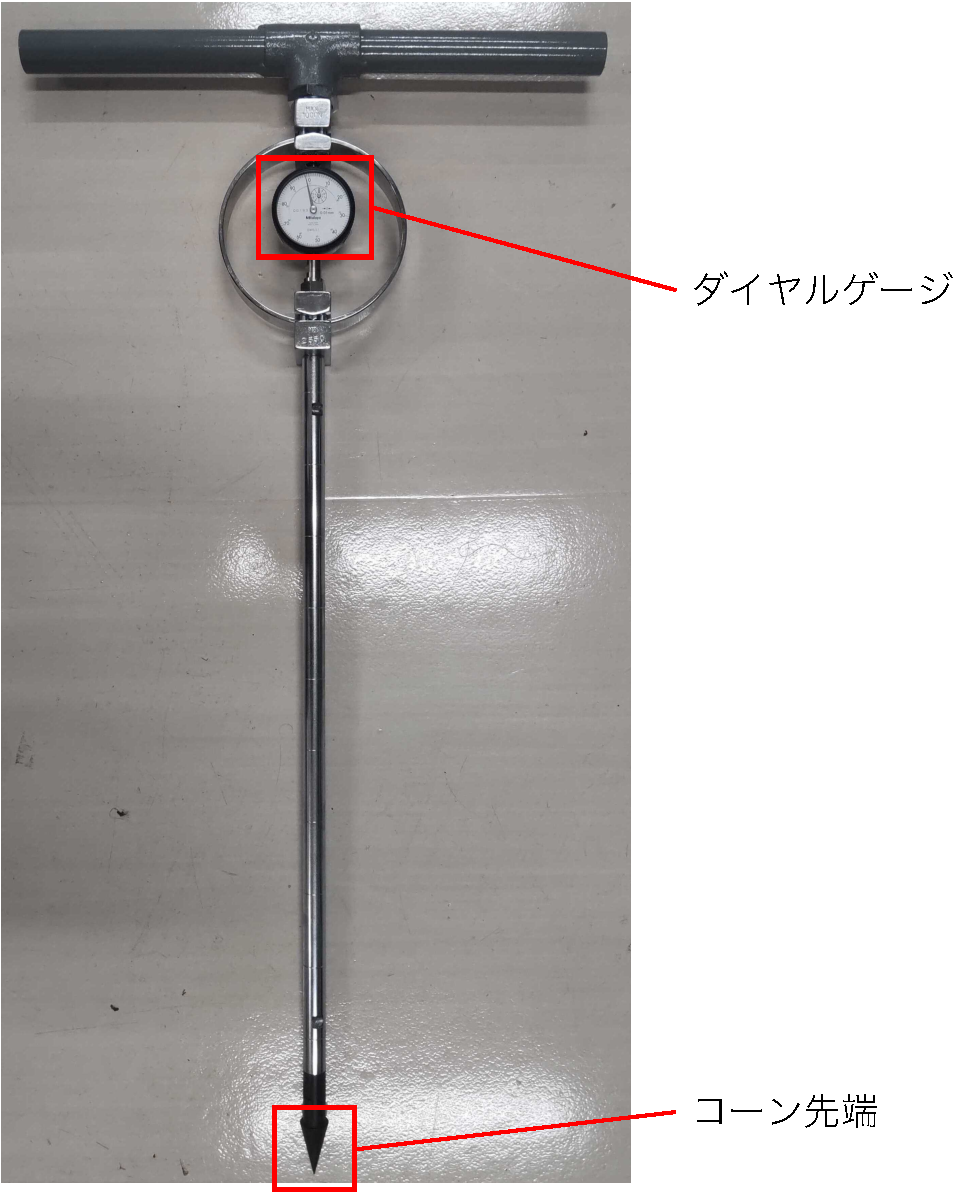
\includegraphics[keepaspectratio, width=0.5\linewidth]{chap1/cone_penetrometer.pdf}
  \caption{コーンペネトロメータ}
  \label{fig:cone_penetrometer}
\end{figure}

% textlint-disable

\vspace{3\zh}
\begin{table}[t]
  \caption{走行に必要なコーン指数(\protect\citeja{maff2015}を基に作成)}
  \label{tab:traffic_cone_index}
  \centering
  \begin{tabular}{cc}
    \toprule
    建設機械の種類                      & コーン指数[\unit{\kN/\m^2}] \\
    \midrule
    超湿地ブルドーザー                    & 200以上                \\
    湿地ブルドーザー                     & 300以上                \\
    普通ブルドーザー(\qty{15}{\tonne}級程度) & 500以上                \\
    普通ブルドーザー(\qty{21}{\tonne}級程度) & 700以上                \\
    スクレープドーザ                     & 600以上                \\
                                 & (超湿地型は400以上)         \\
    被けん引式スクレーパ(小型)               & 700以上                \\
    自走式スクレーパ(小型)                 & 1,000以上              \\
    ダンプトラック                      & 1,200以上              \\
    \bottomrule
  \end{tabular}
\end{table}

% textlint-enable

\clearpage

\section{先行研究}
\label{sec:intro_previous-research}

\clearpage

\section{本研究の目的}
\label{sec:intro_my_purpose}

本研究の目的を以下の通りに設定する.

% textlint-disable ja-technical-writing/ja-no-mixed-period

\bigskip
\begin{itembox}[c]{目的}
  \centering
  目的をここに書く
\end{itembox}

% textlint-enable ja-technical-writing/ja-no-mixed-period

\clearpage

\section{本論文の構成}
\label{sec:configuration}

本論文は,全\ref{cp:conclusion}章から構成されている.
本論文の構成を\reffig{fig:configuration}に示す.

\refcp{cp:introduction}では,本研究の背景と先行研究,目的について述べた.

\refcp{cp:proposed_method}では,提案手法について述べる.

\refcp{cp:verification_experiment}では,\refcp{cp:proposed_method}で述べた提案手法の有効性を確認するための検証実験とその結果,考察について述べる.

\refcp{cp:conclusion}では,本論文の結論と今後の展望を述べる.

\vspace{3\zh}
\begin{figure}[h]
  \centering
  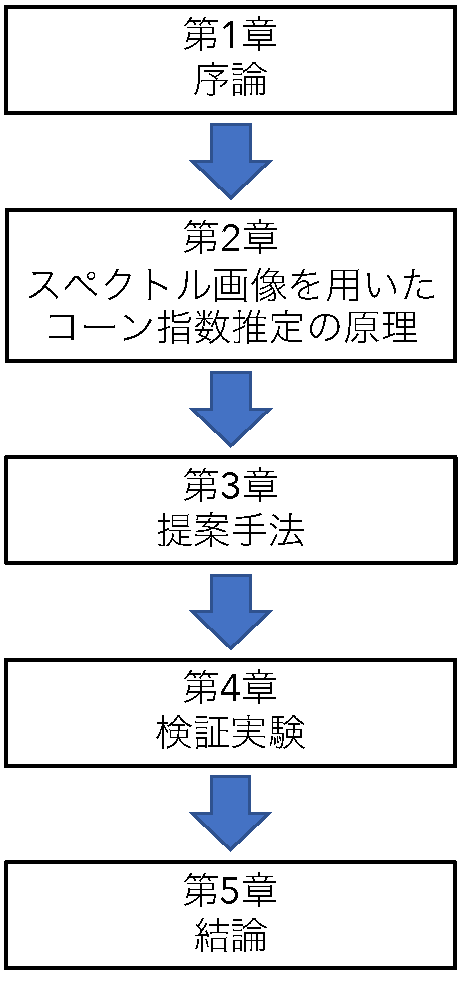
\includegraphics[keepaspectratio, width=0.35\linewidth]{chap1/configuration.pdf}
  \caption{本論文の構成}
  \label{fig:configuration}
\end{figure}

\clearpage

\end{document}
